\documentclass[paper=a4, fontsize=11pt]{article} % A4 paper and 11pt font size

% ---- Entrada y salida de texto -----

\usepackage[T1]{fontenc} % Use 8-bit encoding that has 256 glyphs
\usepackage[utf8]{inputenc}
% \usepackage[light,math]{iwona}

\usepackage{fancyhdr}
\usepackage{fancybox}
\usepackage{pseudocode}


% ---- Idioma --------

\usepackage[spanish, es-tabla]{babel} % Selecciona el español para palabras introducidas automáticamente, p.ej. "septiembre" en la fecha y especifica que se use la palabra Tabla en vez de Cuadro

% ---- Otros paquetes ----

\usepackage{amsmath,amsfonts,amsthm} % Math packages
\usepackage{graphics,graphicx, floatrow} %para incluir imágenes y notas en las imágenes
\usepackage{graphics,graphicx, float} %para incluir imágenes y colocarlas
\usepackage{enumerate}
\usepackage{subfigure}
% \makesavenoteenv{tabular}
% \makesavenoteenv{table}
% Para hacer tablas comlejas
%\usepackage{multirow}
%\usepackage{threeparttable}

\usepackage{sectsty} % Allows customizing section commands
\allsectionsfont{\centering \scshape} % Make all sections centered, the default font and small caps

\usepackage{fancyhdr} % Custom headers and footers
\usepackage[usenames, dvipsnames]{color}
\usepackage{colortbl}

\usepackage{xcolor}
\usepackage{url}

\usepackage{cite}

\usepackage[bookmarks=true,
    bookmarksnumbered=false, % true means bookmarks in
             % left window are numbered
    bookmarksopen=false,   % true means only level 1
             % are displayed.
    colorlinks=true,
    urlcolor=webblue,
    citecolor=webred,
    linkcolor=webblue]{hyperref}
\definecolor{webgreen}{rgb}{0, 0.5, 0} % less intense green
\definecolor{webblue}{rgb}{0, 0, 0.5}  % less intense blue
\definecolor{webred}{rgb}{0.5, 0, 0} % less intense red

%% Define a new 'leo' style for the package that will use a smaller font.
\makeatletter
\def\url@leostyle{%
  \@ifundefined{selectfont}{\def\UrlFont{\sf}}{\def\UrlFont{\small\ttfamily}}}
\makeatother
%% Now actually use the newly defined style.
\urlstyle{leo}

\pagestyle{fancyplain} % Makes all pages in the document conform to the custom headers and footers
\fancyhead{} % No page header - if you want one, create it in the same way as the footers below
\fancyfoot[L]{} % Empty left footer
\fancyfoot[C]{} % Empty center footer
\fancyfoot[R]{\thepage} % Page numbering for right footer
\renewcommand{\headrulewidth}{0pt} % Remove header underlines
\renewcommand{\footrulewidth}{0pt} % Remove footer underlines
\setlength{\headheight}{13.6pt} % Customize the height of the header

\numberwithin{equation}{section} % Number equations within sections (i.e. 1.1, 1.2, 2.1, 2.2 instead of 1, 2, 3, 4)
\numberwithin{figure}{section} % Number figures within sections (i.e. 1.1, 1.2, 2.1, 2.2 instead of 1, 2, 3, 4)
\numberwithin{table}{section} % Number tables within sections (i.e. 1.1, 1.2, 2.1, 2.2 instead of 1, 2, 3, 4)

\setlength\parindent{0pt} % Removes all indentation from paragraphs - comment this line for an assignment with lots of text

\newcommand{\horrule}[1]{\rule{\linewidth}{#1}} % Create horizontal rule command with 1 argument of height

%%%%% Para cambiar el tipo de letra en el título de la sección %%%%%%%%%%%
% \usepackage{sectsty}
% \chapterfont{\fontfamily{pag}\selectfont} %% for chapter if you want
% \sectionfont{\fontfamily{pag}\selectfont}
% \subsectionfont{\fontfamily{pag}\selectfont}
% \subsubsectionfont{\fontfamily{pag}\selectfont}

%----------------------------------------------------------------------------------------
% TÍTULO Y DATOS DEL ALUMNO
%----------------------------------------------------------------------------------------

\title{ 
\normalfont \normalsize 
\textsc{{\bf Redes y Sistemas Complejos (2016-2017)} \\ Grado en Ingeniería Informática \\ Universidad de Granada} \\ [25pt] % Your university, school and/or department name(s)
\horrule{0.5pt} \\[0.4cm] % Thin top horizontal rule
\huge Memoria Práctica 1 \\ Análisis Preliminar y Visualización Básica de una Red de Facebook con Gephi\\% The assignment title
\horrule{2pt} \\[0.5cm] % Thick bottom horizontal rule
}

\author{Braulio Vargas López\\DNI: 20079894C\\Correo: brauliovarlop@correo.ugr.es} % Nombre y apellidos

\date{\normalsize\today} % Incluye la fecha actual

%----------------------------------------------------------------------------------------
% DOCUMENTO
%----------------------------------------------------------------------------------------

\begin{document}

\maketitle % Muestra el Título
\pagenumbering{gobble}
\newpage %inserta un salto de página

\tableofcontents % para generar el índice de contenidos
% \newpage
\pagenumbering{arabic}

\section{Red del grupo, visualización y datos}

La red utilizada es la que se encuentra en el grupo de Facebook \href{https://www.facebook.com/groups/goteborgerasmus1314/?fref=ts}{GOTEBORG ERASMUS 2013/2014}. En el momento en que se descargaron los datos, el grupo constaba de 2720 miembros de distintos países de Europa y se descargaron los datos de 800 posts del grupo, en los que aparecen las conexiones entre los usarios del grupo.

A continuación podemos ver la red completa que conforma el grupo. Una red con 1014 nodos y 1050 enlaces entre ellos. Esta red tiene una gran componente conexa, pero a la vez, tiene un montón de islas que podemos ver entorno a la componente gigante de la red. En ella podemos ver la red distribuida gracias al algoritmo \textbf{Force Atlas 2}, donde los nodos más grandes son aquellos que mayor valor de intermediación tiene, haciendo de puente entre las pequeñas comunidades del mapa. El color nos lo da el valor de la centralidad del vector propio, siendo más rojos los nodos más centrales según su centralidad del vector propio.

\begin{figure}[H]
  \centering
  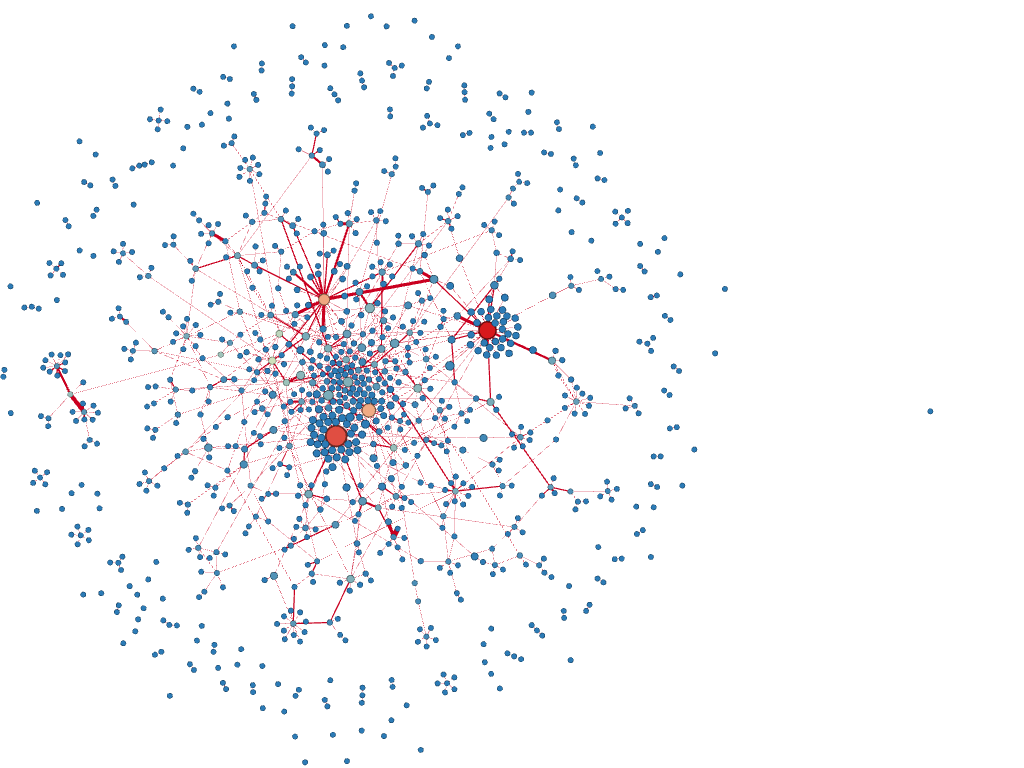
\includegraphics[scale=0.225]{RedCompleta}
  \caption{Red completa}
  \label{red_cmp}
\end{figure}

\begin{figure}[H]
  \centering
  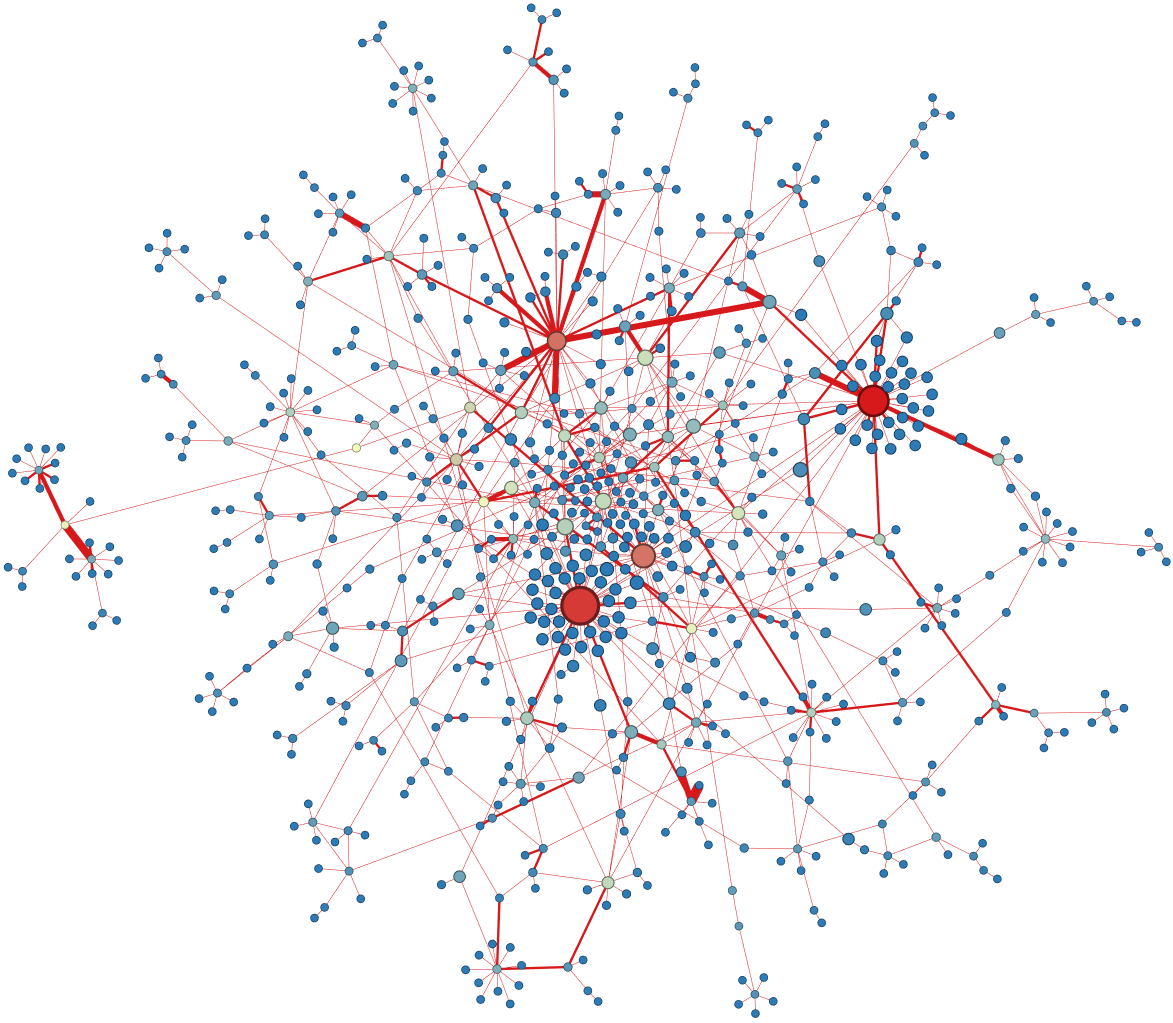
\includegraphics[scale=0.225]{componente_gigante}
  \caption{Componente gigante}
  \label{giant}
\end{figure}

\begin{center}  
\begin{tabular}{|c|c|}
\hline
\textbf{Medida} & Valor \\
\hline
Número de nodos $N$ & 1014 \\
\hline
Número de enlaces $L$ & 1050 \\
\hline
Número máximo de enlaces $L_{max}$ & 512578 \\
\hline
Densidad del grafo $\frac{L}{L_{max}}$ & 0,002048468720858 \\
\hline
Grado medio $<k>$ & 1,92 \\
\hline
Diámetro $d_{max}$ & 13 \\
\hline
Distancia media $d$ & 5,468 \\
\hline
Coeficiente medio de clustering $<C>$ & 0,022 \\
\hline
Número de componentes conexas & 164\\
\hline
Número de nodos componente gigante (y \%) & 749 (73,87) \\
\hline
Número de aristas componente gigante (y \%) & 948 (90,29) \\
\hline  
\end{tabular}
\end{center}

\subsection{Gráficos asociados a los datos}

\begin{figure}[H]
    \centering
    \mbox {
        \subfigure[Distribución de grados de la red]{
        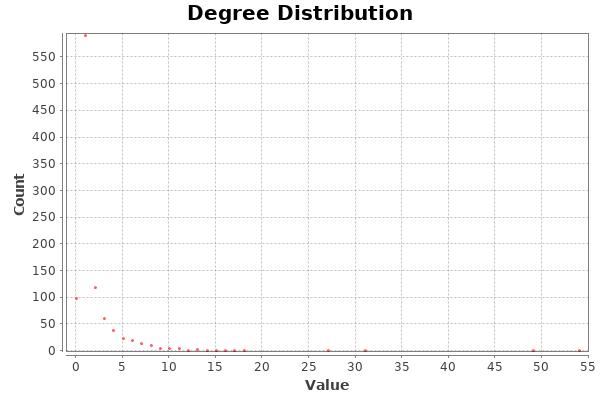
\includegraphics[width=0.5\textwidth]{./GradoMedio/degree-distribution}
        \label{degree}
      }
      \qquad
      \subfigure[Coeficiente de clustering de la red] {
        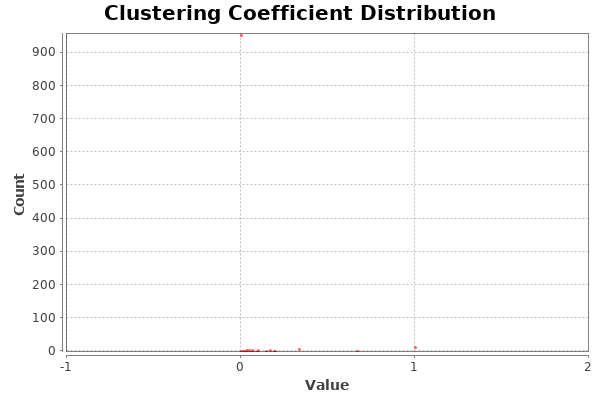
\includegraphics[width=0.5\textwidth]{./CoeficienteClustering/clustering-coefficient}
        \label{cluster}
        }
    }
    \mbox {
        \subfigure[Distribución de la intermediación de los nodos en la red]{
        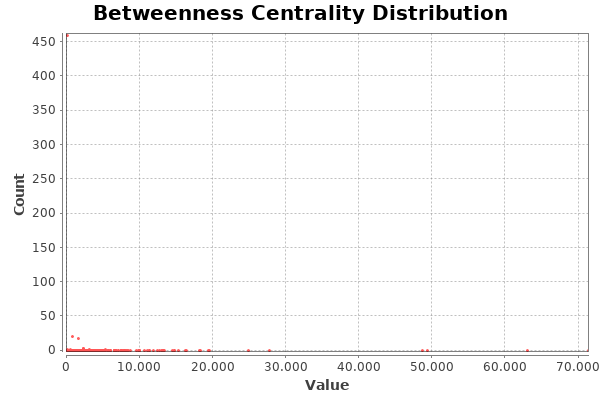
\includegraphics[width=0.5\textwidth]{./Diametro_red/BetweennessCentralityDistribution}
        \label{between}
      }
      \qquad
      \subfigure[Excentricidad de los nodos de la red] {
        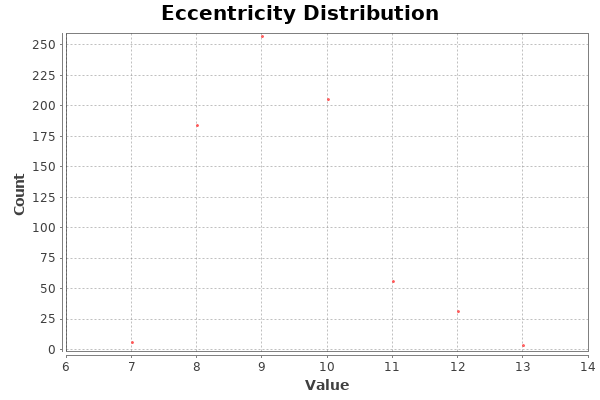
\includegraphics[width=0.5\textwidth]{./Diametro_red/EccentricityDistribution}
        \label{eccentricity}
        }
    }
    \caption{Diferentes medidas usadas en la red}
    \label{medidas}
\end{figure}

\section{Descripción}

Como podemos ver en los datos y en la tabla, tenemos una gran red de 1014 nodos en total. En esta red, existen 164 componentes conexas, habiendo una sola componente gigante que supone el 73.87\% de los nodos totales de la red, mientras que el resto de componentes, podemos ver cómo se situan alrededor de esta. 

La distribución de color corresponde al valor de intermediación de los nodos, siendo menos centrales los nodos de color azul, y cuanto más rojo, más central es el nodo, mientras que a mayor tamaño, más central es el nodo. Como se puede ver, existen varios nodos centrales, que son los que conenctan la mayoría de nodos de la componente gigante, entre sí. Además, las aristas que salen de estos nodos son de mayor tamaño ya que, a mayor número de interacciones entre los usuarios, mayor es el peso de la arista. 

\end{document}


nodo ---> eigenvector centrality
color -->betweeness centrality

